\documentclass{article}

\usepackage{arxiv}

\usepackage[utf8]{inputenc} % allow utf-8 input
\usepackage[T1]{fontenc}    % use 8-bit T1 fonts
\usepackage{hyperref}       % hyperlinks
\usepackage{url}            % simple URL typesetting
\usepackage{booktabs}       % professional-quality tables
\usepackage{amsfonts}       % blackboard math symbols
\usepackage{nicefrac}       % compact symbols for 1/2, etc.
\usepackage{microtype}      % microtypography
\usepackage{cleveref}       % smart cross-referencing
\usepackage{graphicx}
\usepackage{natbib}
\usepackage{doi}
\usepackage{todonotes}
\usepackage{caption}
\graphicspath{{./images/}}


\title{Super-resolution image reconstruction for Earth observation}

\date{May 12, 2022}

\author{Casey Primel}

\renewcommand{\headeright}{Project Report}
\renewcommand{\undertitle}{Project Report}
\renewcommand{\shorttitle}{Super-resolution image reconstruction}


\begin{document}
\maketitle

\begin{center}
    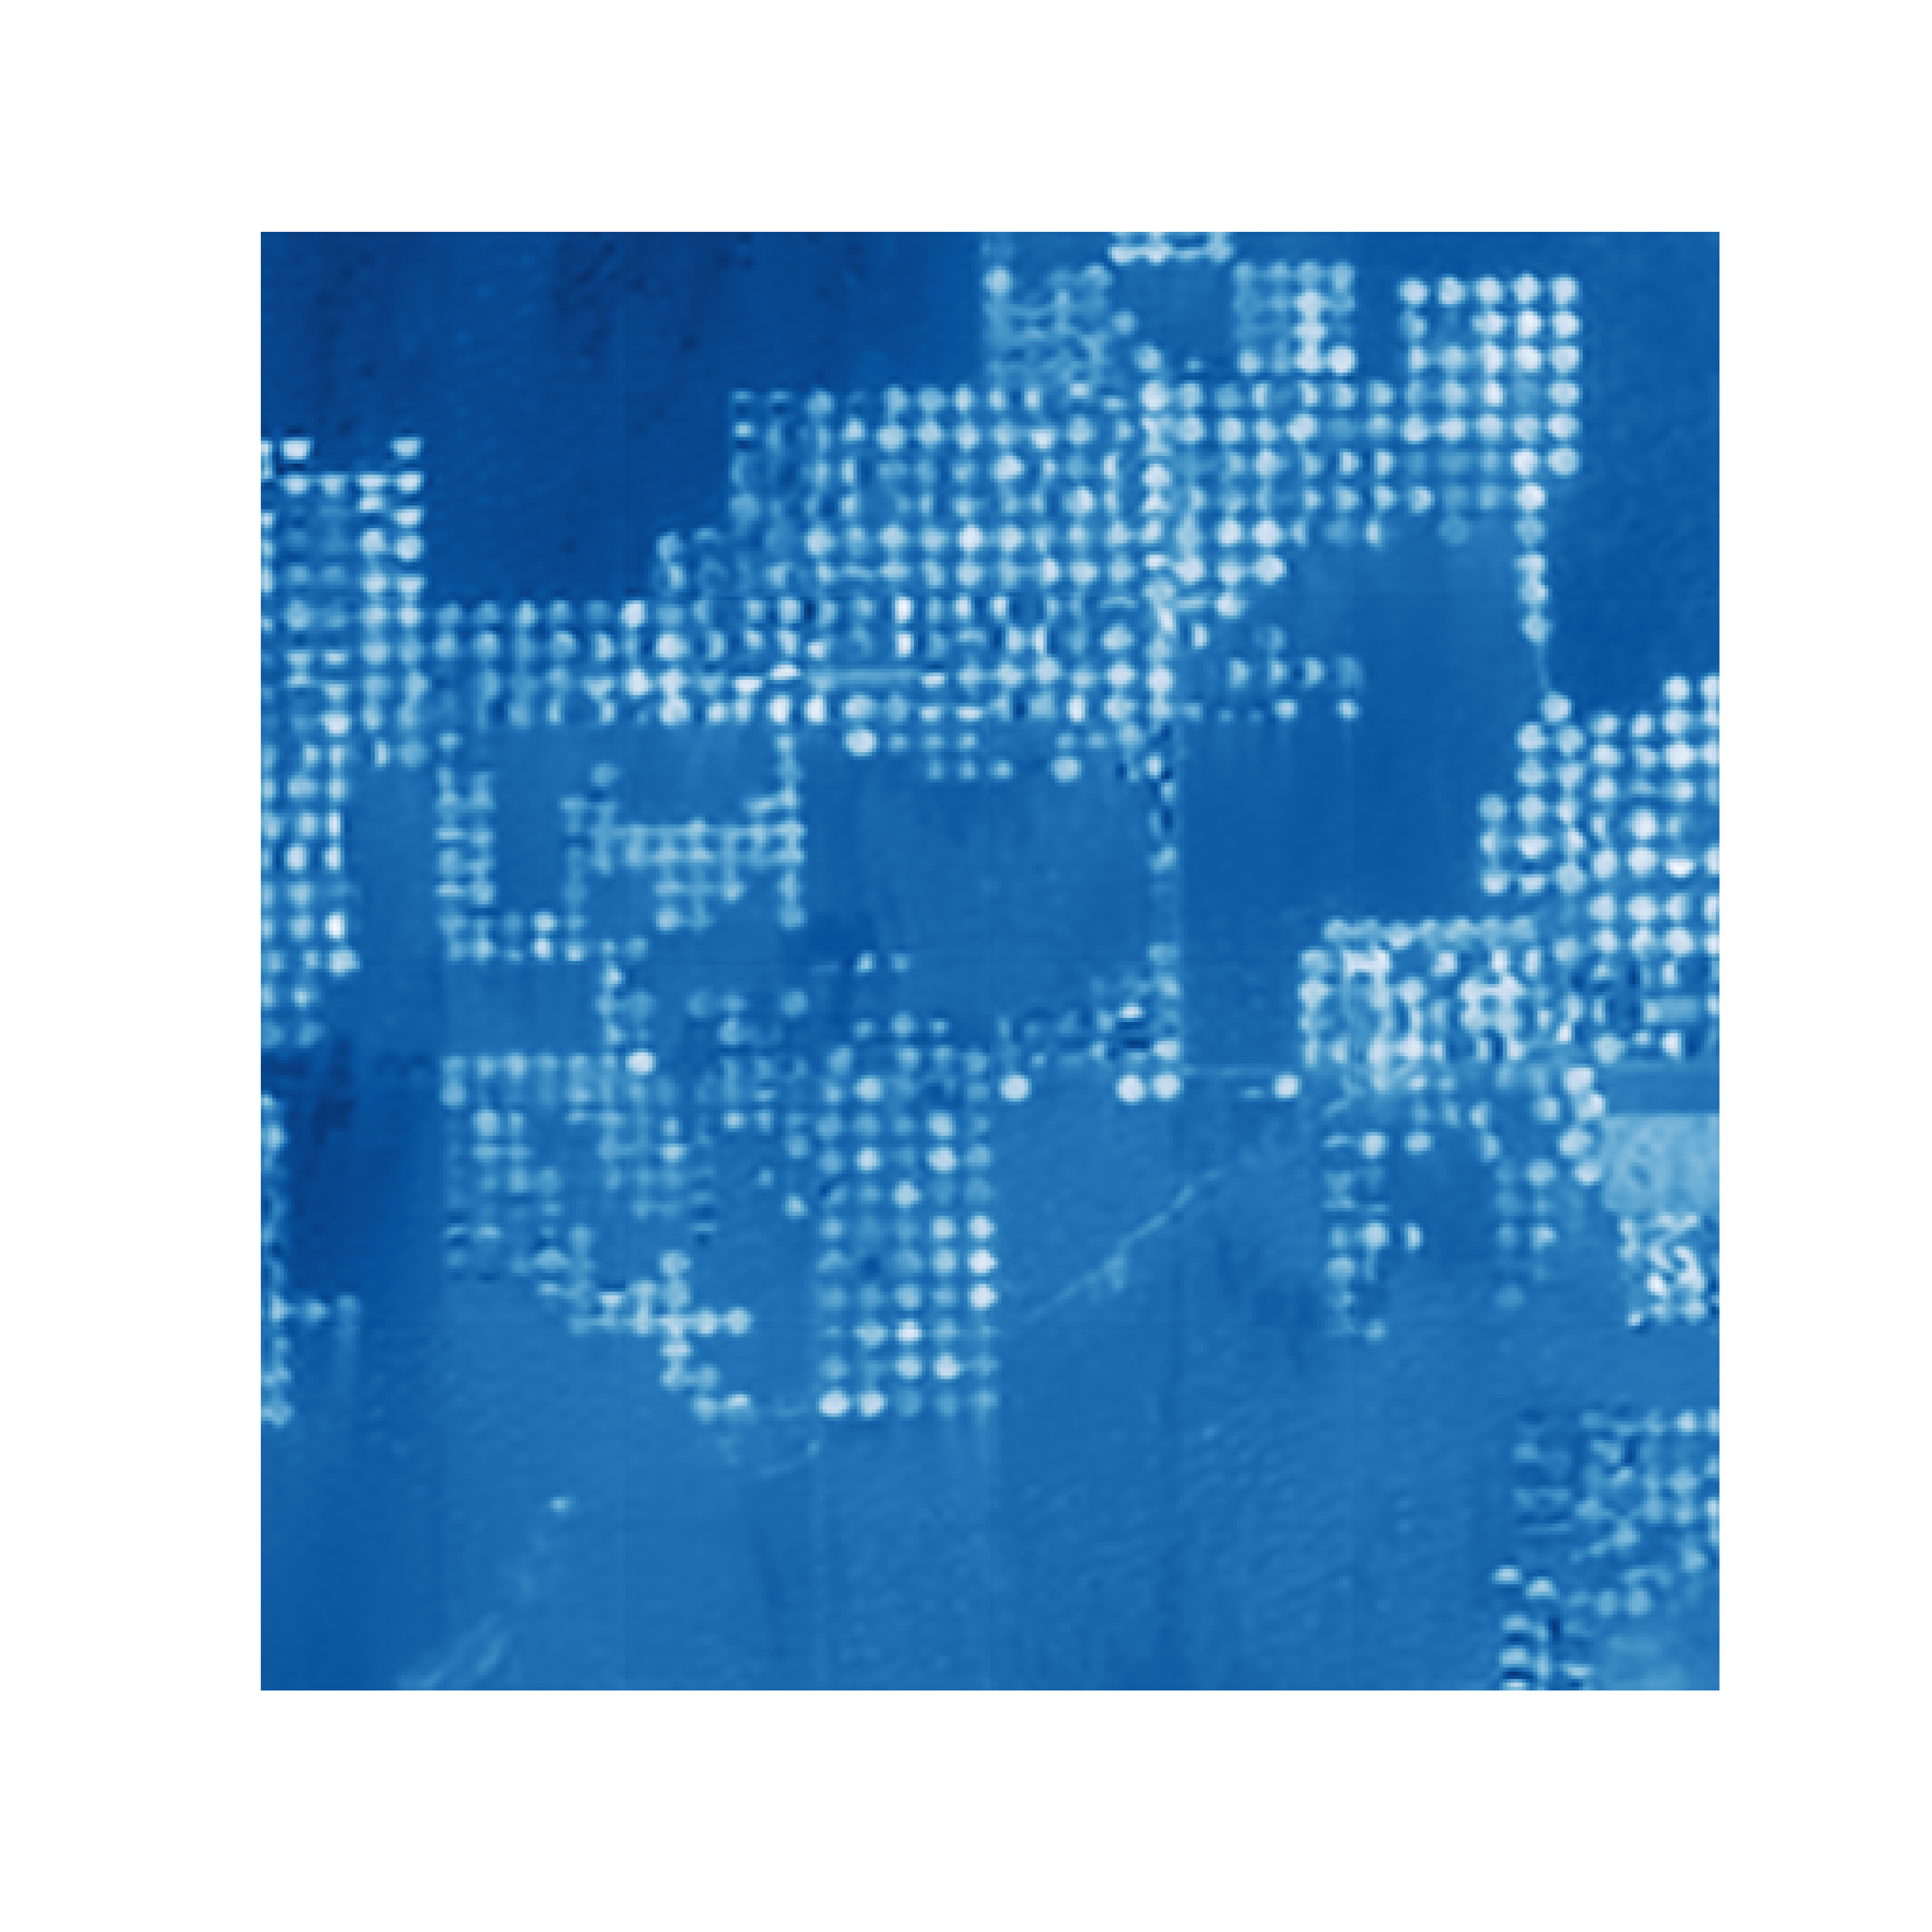
\includegraphics[width=0.75\textwidth]{superres2.png}
    \captionof{figure}{These fields do not exist... sort of: A super-resolved 384x384 pixel image outputted by a WDSR-3D network from a low-resolution 128x128 image set.}
\end{center}



\section{Introduction}

This project takes as its starting point the prompt and dataset provided by \citet{Martens2021} which served as the basis of the European Space Agency's Advanced Concepts Team's PROBA-V Super Resolution challenge in 2019.\footnote{https://kelvins.esa.int/proba-v-super-resolution/} The challenge was run to test the performance of MISR methods for post-processing of satellite images taken over a period of multiple days. Without exception, submissions were built around convolutional neural network architectures, e.g., the winning submission from \citet{Molini2020}. Postmortem submissions showed improvements by formalizing the MISR problem as SISR on video frames, incorporating time as an additional dimension of information \citep*{mark_bajo_2020_3733116,Dorr2020}. The models proposed by the latter have the added benefit of being less complex and capable of being practically run on a single GPU.

The aim of the project is to replicate and attempt to extend on existing solutions, in particular the modified WDSR network architecture proposed by\citet{Dorr2020} and \citet{mark_bajo_2020_3733116}. The proposed contribution involves the fine-tuning of the initial SR model by training it as a generator in a generative adversarial network. This technique, first proposed by \citet{Ledig2016} for SISR, works by incorporating an additional notion of a perceptual loss on top of the pixel-wise loss used to train the initial SR model. In other SISR applications, this has resulted in significant gains to perceptual quality. As indicated by \citet{Zhao2017}, mixing pixel-wise and perceptual loss can lead to better results even when measured against metrics that do not take into account human perception. The question one would want to answer here is whether such a technique can also be used to improve results in the specific context of EO imagery.

Unfortunately, while we were able to implement and replicate the results of the first, we were not able to implement a working solution for incorporating the WDSR3D network architecture into a generative adversarial network. These difficulties and suggested paths forward are discussed more fully in the conclusion.

\section{Background}

Super-resolution image reconstruction (SR) refers to algorithms for obtaining a high-resolution image from a single or multiple low-resolution images by increasing the number of pixels per unit area in an image. SR is especially important in context where hardware-based solutions, e.g., increasing the sensor size or decreasing the pixel size, are prohibitively expensive or impractical. As a result, SR finds many use cases from smartphones to Earth observation satellites. SR methods fall into two broad categories, frequency and spatial. We can further distinguish between single image (SISR) and multiple image SR (MISR) \citep{Nasrollahi2014}. As the names imply, SISR obtains a high-resolution image from a single low-resolution input and MISR from multiple low-resolution inputs. Another important distinction is in their outputs: whereas SISR methods require imputing "lost" pixels to generate their high-resolution outputs, MISR can mobilize subpixel differences to maintain the linkage between imputed pixel values and real observations \citep{Martens2021}.

Our project focuses on MISR in the context of earth observation (EO) imagery. The problem in EO is, simply put, there is a high availability of low-resolution images but low availability of high-resolution images for any given location over a particular time period. In many cases, the images might come from successive passes of a satellite over the same coordinates leading to differences in illumination, cloud cover and actual image content. In other cases, the images might be an instantaneous multi-spectral snapshot of a location produced from separate instruments of the same satellite on a single pass. From this data, one needs to generate a series of images with temporal and spatial resolutions adequate to the problem at hand. For example, given a low-resolution image for a particular date and two high-resolution images taken close to that date, one needs to derive a single high-resolution for the given date. Within remote sensing, this is accomplished through methods of spatio-temporal fusion: "fusing" temporally dense, coarse resolution images and temporally sparse, high-resolution images. MISR, in contrast, aims to produce a single high-resolution output from only low-resolution inputs.


\section{Methodologies}

The project is implemented in Python, using NumPy and Tensorflow libraries for array manipulation and model training. The \verb|phase_cross_correlation| function from \verb|skimage| was used for performing image registration.\footnote{I had originally intended to use a self-written function for phase cross correlation; however, to attain the same performance, I found myself more or less replicating the work that was already available in skimage (i.e., using fast fourier transforms for the convolution). The choice was made to use the skimage function both for the sake of time and correctness.} 

Many of the teams which submitted a solution to the PROBA-V challenge have made their code public. All of them require access to GPUs and, in most cases, high-memory GPUs. Resources available include data loaders for the dataset and various network architectures. These served as useful references for the project, especially because of the specialized nature of the domain. When appropriate, I make mention and cite any code which is not original.

In terms of hardware, model training was conducted on a cloud-based GPU instance (Google Colab). This is an unfortunate obstacle to replication for this project as well as for large vision models more generally.

A notebook containing all of the code and instructions for running the code can be found at \url{https://colab.research.google.com/drive/19Jhw5tp1cSMGO3QzcfUT5VMkQKVZP9GE?usp=sharing}.


\section{Data}

The dataset is publicly available from the PROBA-V Super Resolution challenge portal. It consists of satellite data from 74 regions. It includes reflectances for the red and near infrared spectral bands\footnote{These bands are used to compute a normalized difference vegetation index to asses and identify different kinds of land cover and land usage.} at 300 meter and 100 meter resolutions. The 300m resolution data is provided as 128x128 grayscale pixel images and the 100m as 384x384 grayscale pixel images. Each image also includes a quality map which indicates which pixels in the image are concealed (e.g., by cloud cover) and which are clear. There are 1450 scenes in the dataset, each containing an average of 19 different low-resolution images. More details can be found on the challenge website.\footnote{https://kelvins.esa.int/proba-v-super-resolution/data/}

\begin{center}
    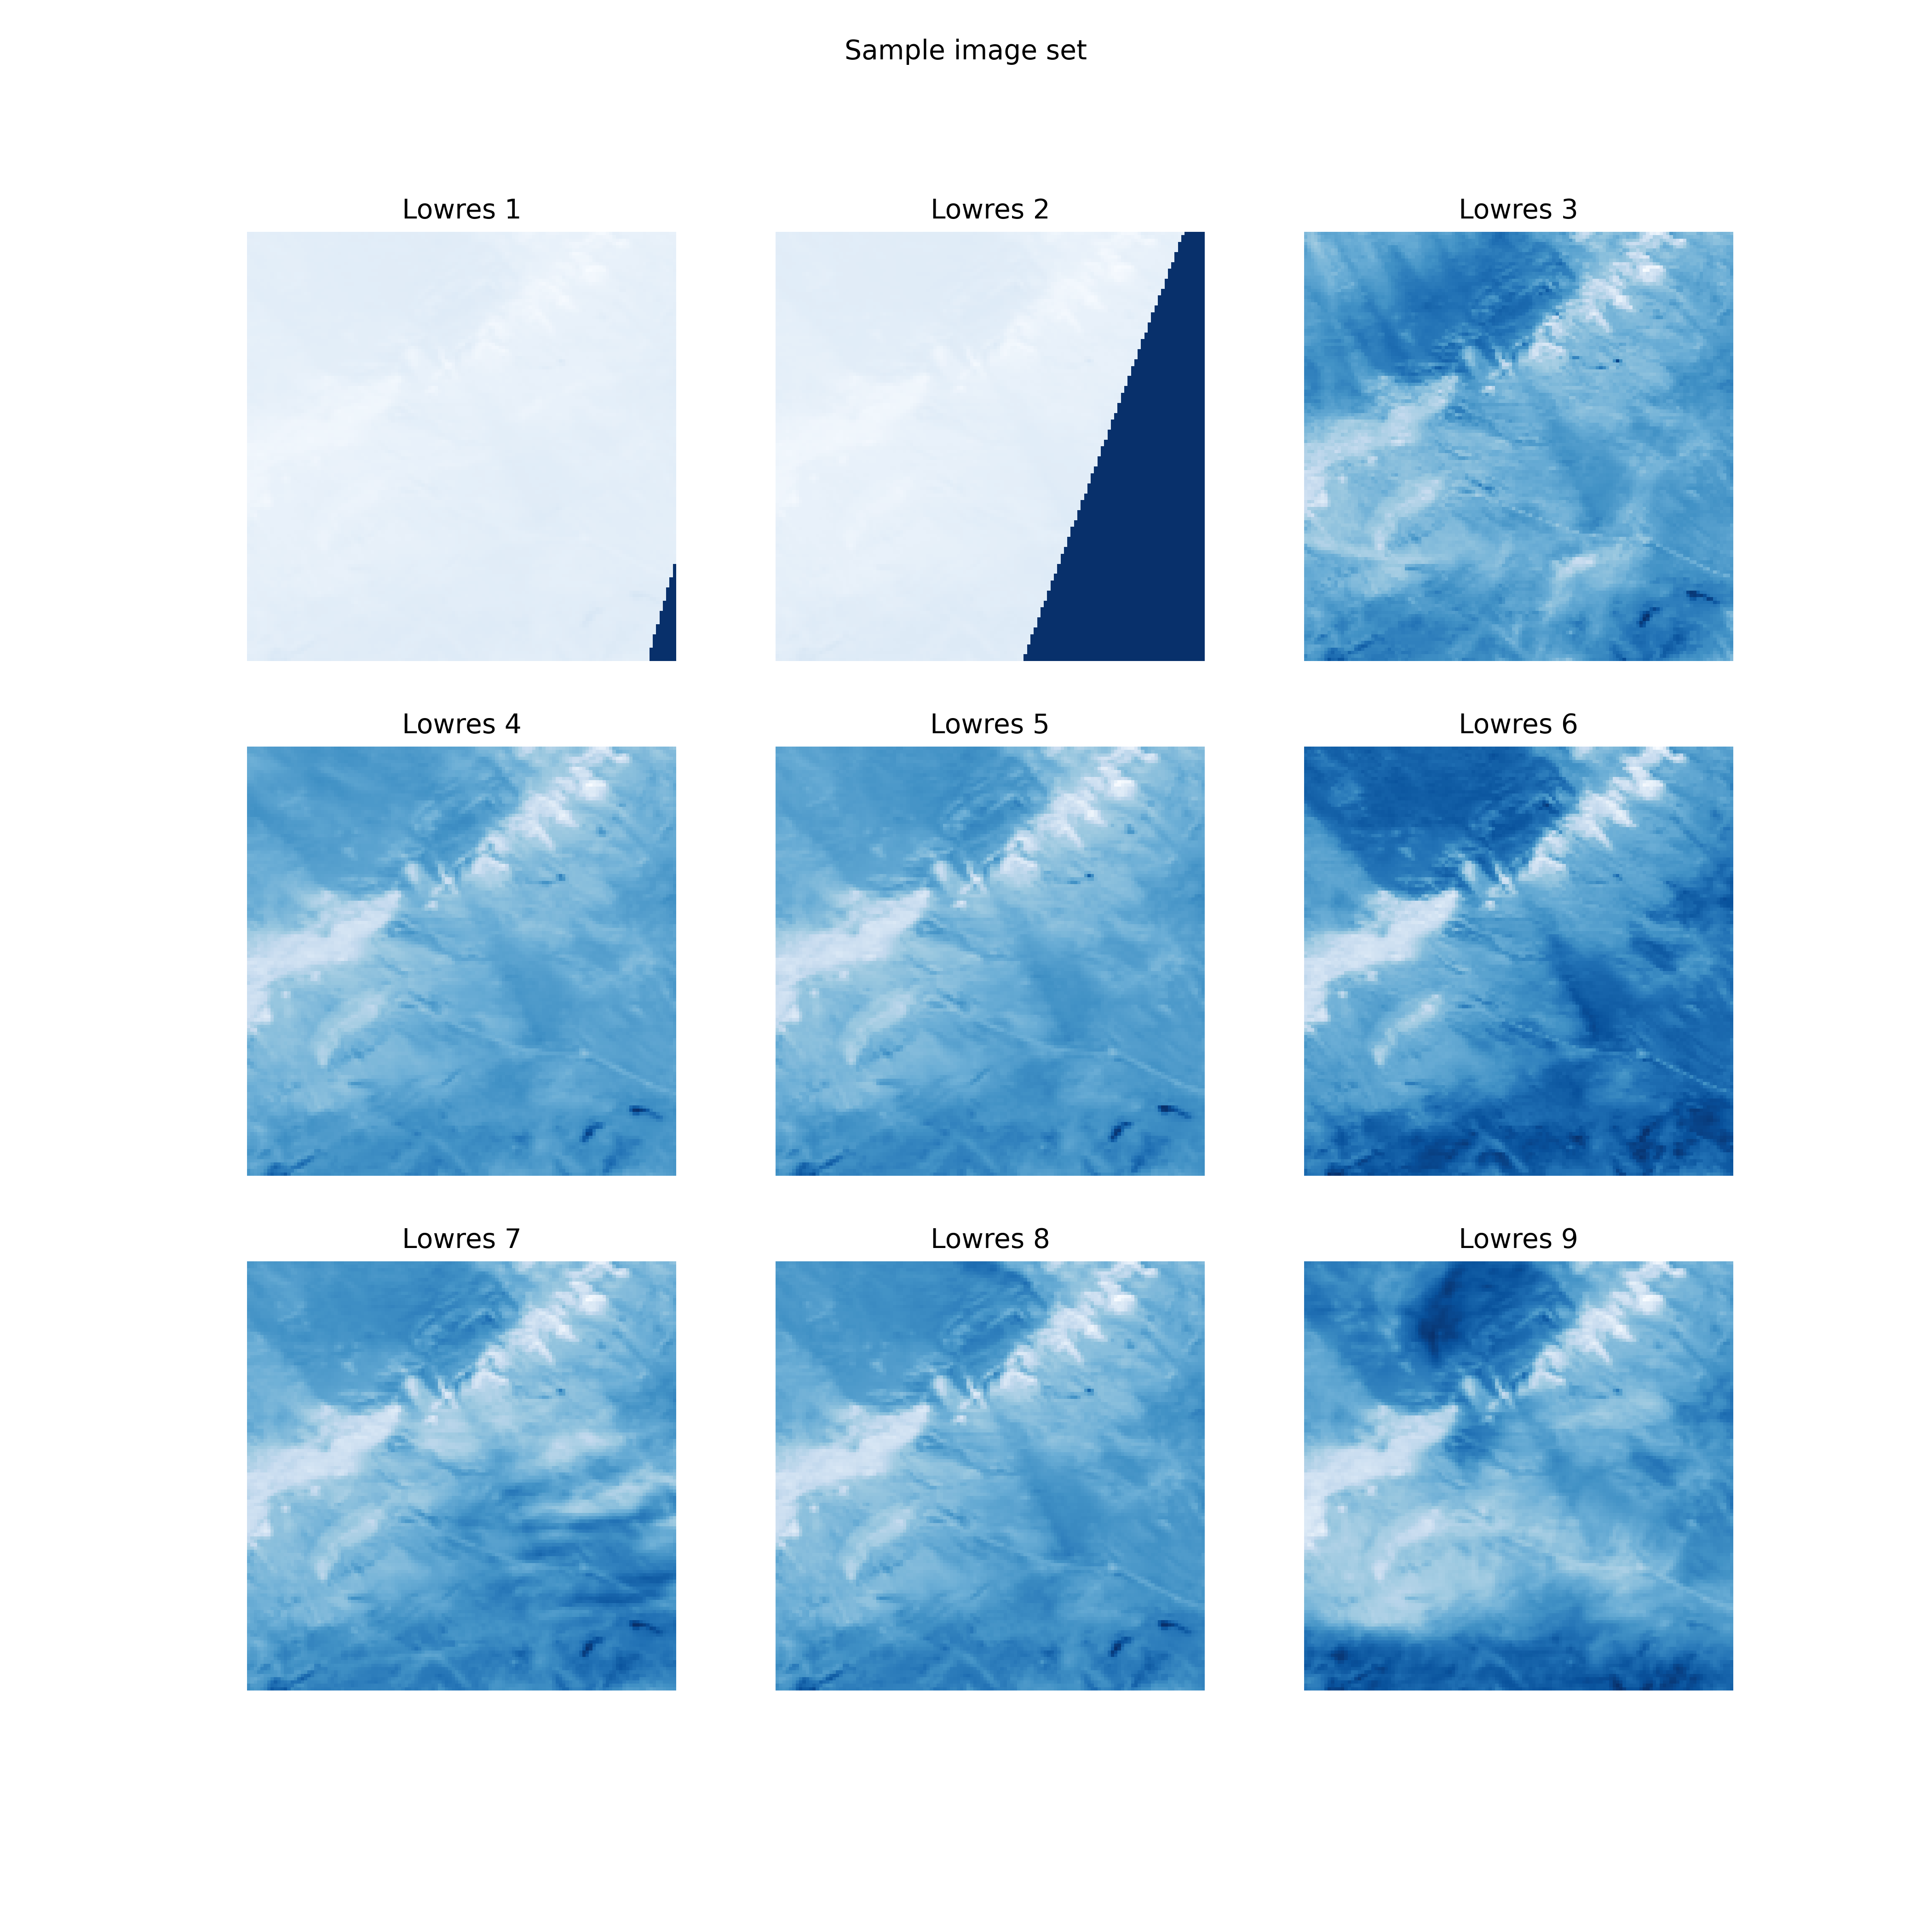
\includegraphics[width=.4\textwidth]{images/sample_image_set.png}
    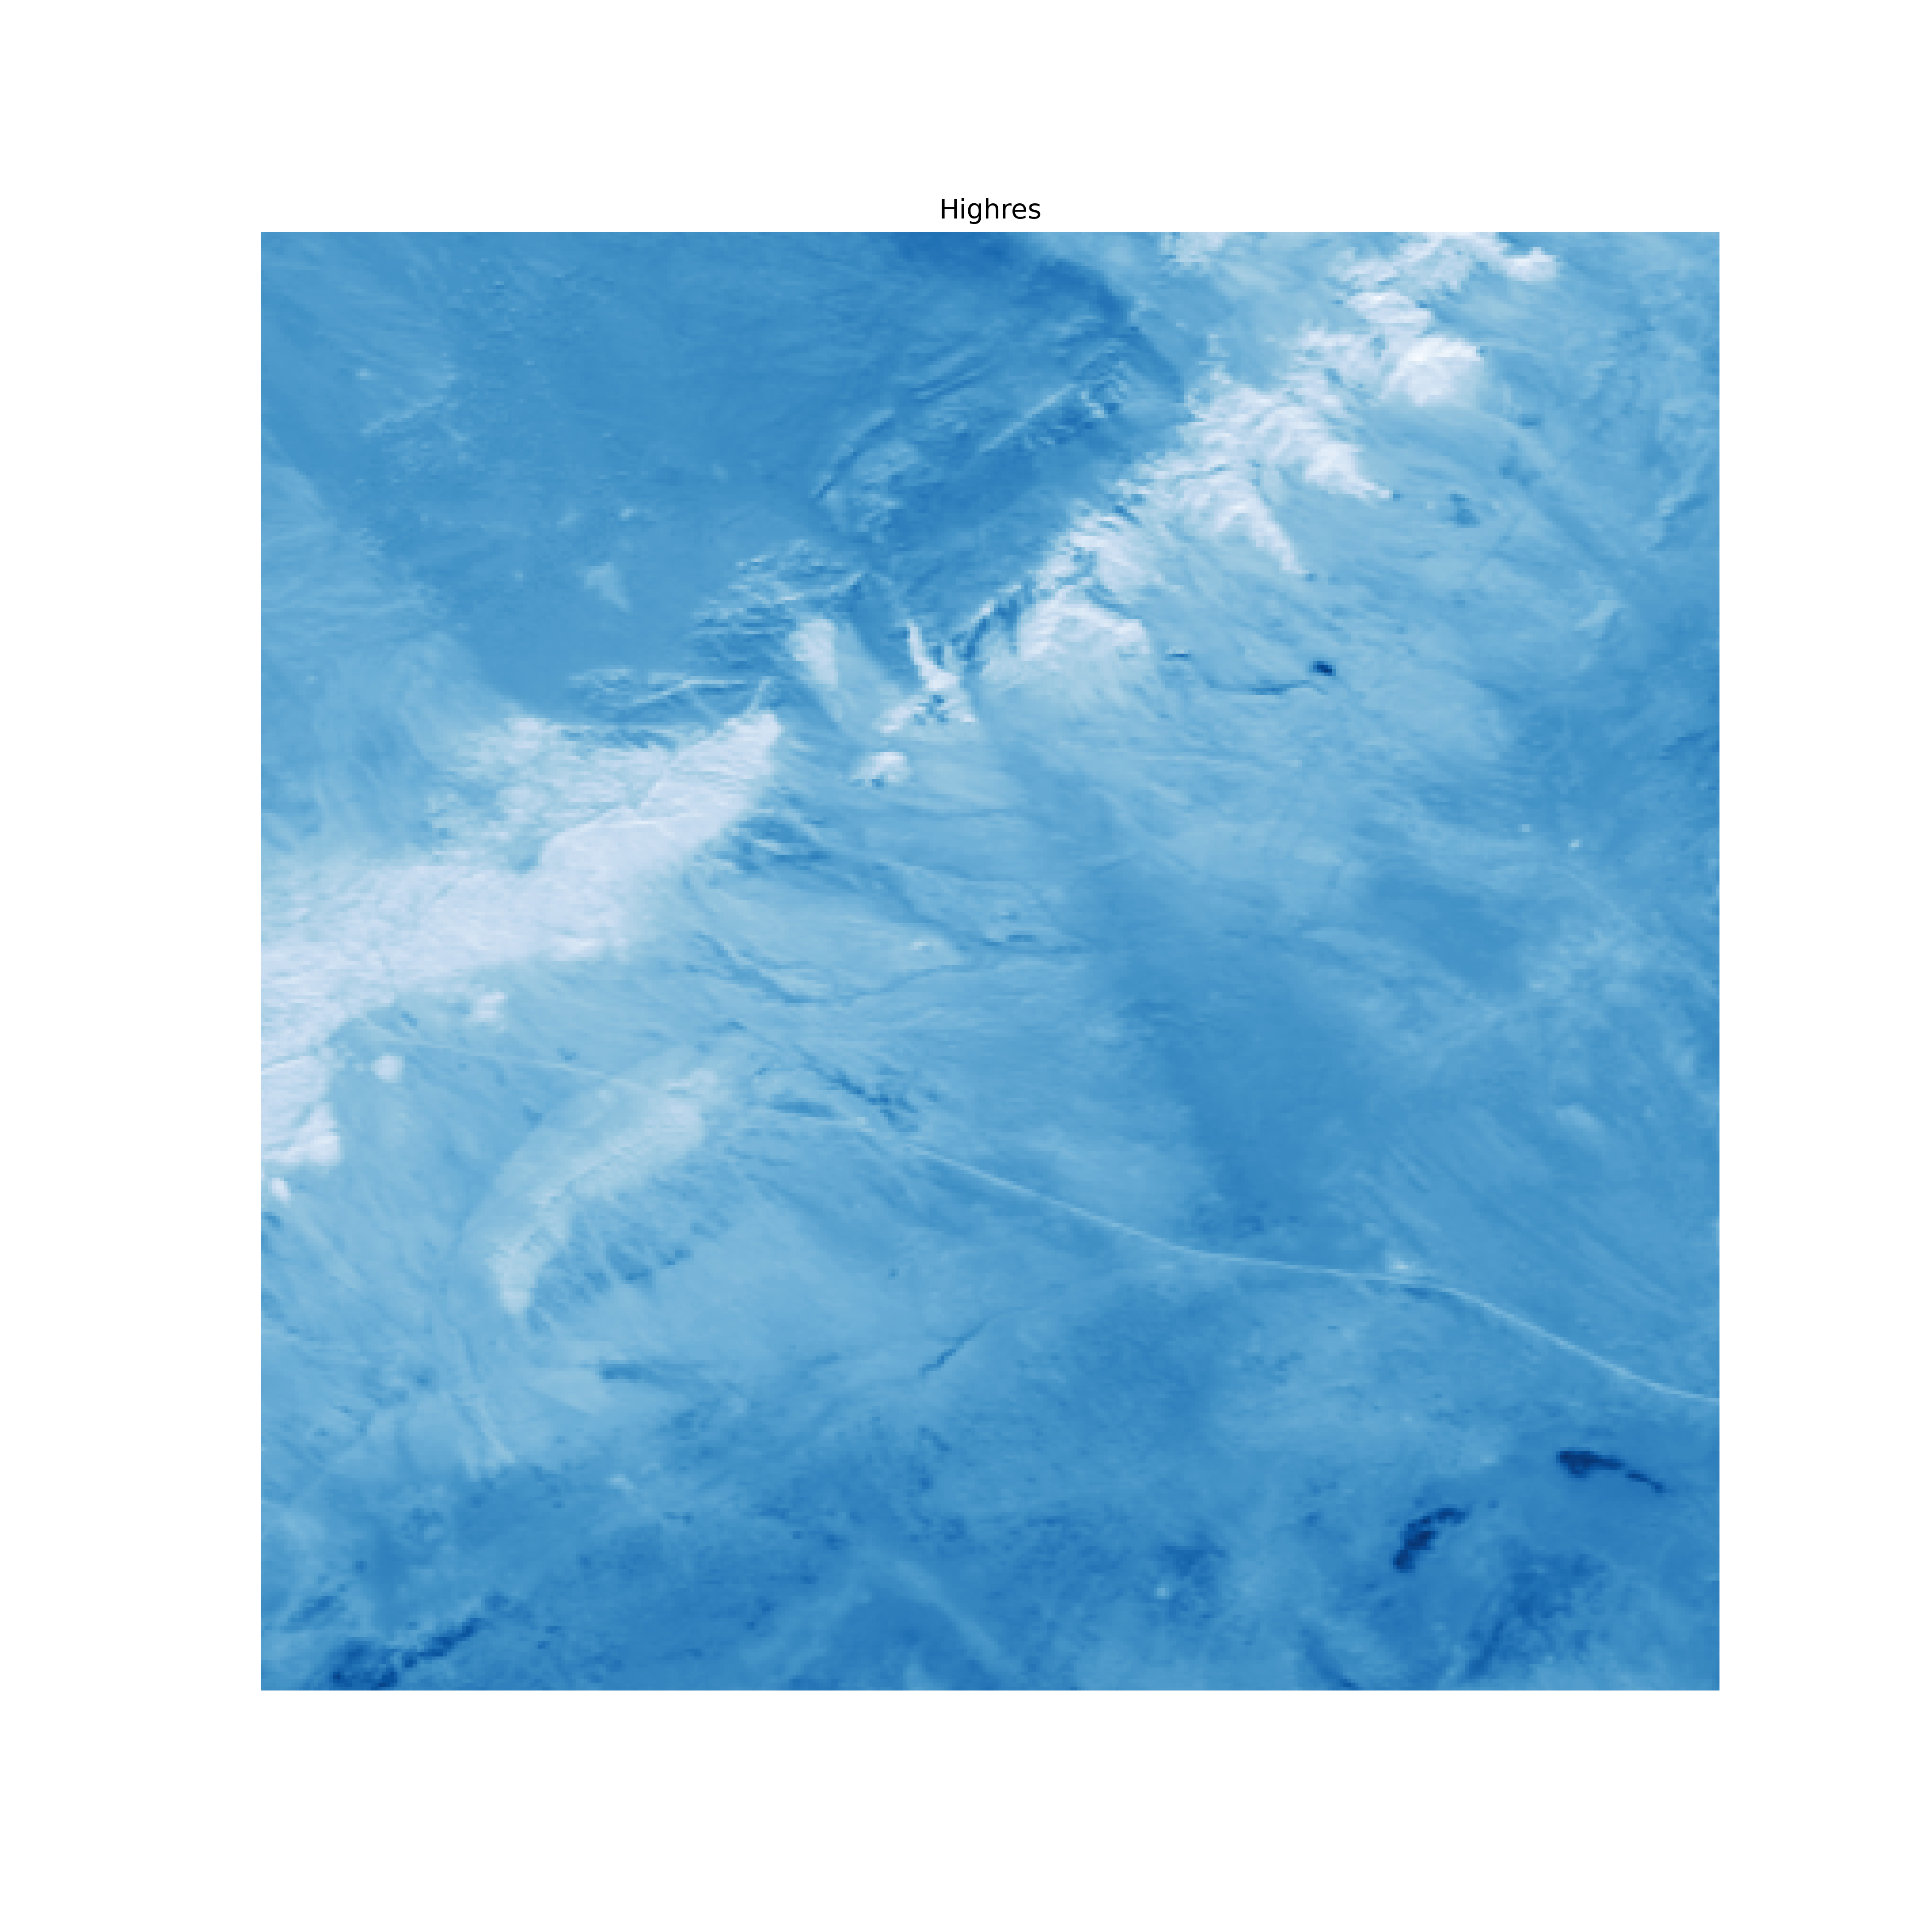
\includegraphics[width=.4\textwidth]{images/sample_hr_target.png}
    \captionof{figure}{Sample low resolution (128x128) image set and high resolution (384x384) target from PROBA-V training data.}
\end{center}

For reason of time and available resources, we will also limit ourselves to the NIR data. This choice will most certainly decrease the performance of our initial model but will allow quicker experiment iteration and be more readily reproducible.


\section{Image preprocessing}

Our initial training data consists of a series of low resolution image sets, their respective high resolution image, and the quality masks associated with each. Several steps are taken to prepare the data for input to the model. During preprocessing, available main memory actually ended up being a major bottleneck. Therefore, the preprocessing pipeline is divided into 3 parts: pickling the image date as \verb|numpy| arrays, loading that data and running it through the preprocessing routine. At each stage of the pipeline, the results are saved to disk so that the pipeline can be resumed if needed. 

The preprocessing routine itself involves 6 steps each of which is detailed below.

\subsubsection{Step 1: Image registration}

Registration methods fall into two domains: spatial and frequency. Spatial works on images and typical works by matching features or intensity patterns in a pair of images and then calculating the offset between them. Frequency methods, as the name implies, operate on a frequency representation of the images. 

For this project, a frequency-domain method, phase correlation, was used to register the images. Phase correlation is standard for geospatial imagery and other domains because it is resilient to noise and other common factors. Registration is performed on the image sets contained in the training and test sets. For each set of images, the clearest image is used as the reference. 

\subsubsection{Step 2: Cleaning image sets}

Cloud cover and other obstructions significantly diminish the usefulness of images for most geospatial image tasks, especially those like calculating NDVI which relies on the reflectance of particular bandwidths. Of course, such obstructions are ubiquitous and we cannot expect to have an image set containing nothing but perfectly clear images. One can easily imagine that it would be hard to produce a super-resolution image from highly obstructed images.

The dataset includes a mask for each image that reports its pixel-level clearance: 1.0 indicates total obstruction and 0.0 perfect visibility. For this project, we have chosen a threshold of $p=0.15$, i.e., we want our images to be no more than 15\% obstructed. All images that do not meet this threshold are discarded.

\subsubsection{Step 3: Selecting best frames}

Even filtering for obstructed images, we can further improve the quality of our output by limiting our image sets to the $k$ best images from each. In our case, we will be using a value of 7. 

\subsubsection{Step 4: Shuffling frames}

 Next we shuffle the order of the frames in each image set. This makes it so that our network does not see images in the same order every time and is directly analogous to shuffling the order of image inputs for other networks.  

\subsubsection{Step 5: Divide images into patches}

Rather than feeding the network whole 128x128 pixel images, we will be creating a series of 34x34 pixel patches from each image. For each image, we construct 16 patches by sliding a window across the image, taking a patch and applying a padding to each side. This has the double benefit of not only diversifying the input data but also increasing the size of the training data.

\subsubsection{Step 6: Mean frames for residual pathway}

The WDSR3D network we are using has a residual path that applies a convolutional layer to the mean image of the image set being propagated through the network. Here, we create an additional array with the means for all the image sets, so it can be added to the training data.

\section{WDSR-3D network architecture}

The WDSR-3D network used here is based off that formulated by \citet{Dorr2020} and \citet{mark_bajo_2020_3733116} for the PROBA-V challenge. Both authors adapted the framework proposed by \citet{kim20183dsrnet} for video superresolution by swapping out its internal 3D convolution layers for WDSR-B blocks \citep{yu2018wide} which use a residual path back to the original low resolution frame--here, the mean of those frames--with a 2D convolution layers applied to it. The result is a smaller network, in terms of parameter size, which requires less memory to train and is still able to outperform larger models for the same task.


\begin{center}
    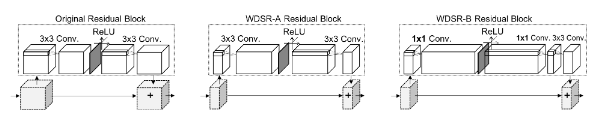
\includegraphics[width=\textwidth]{images/wdsr.png}
    \captionof{figure}{Comparison of residual network with original residual blocks versus WDSR residual blocks. From Kim et al.}
\end{center}



\subsection{Loss and accuracy functions}

A modified L1 loss function is used for training the network and a modified peak signal-to-noise ratio (PSNR)\footnote{$PSNR = 10 * \log_{10} \frac{MAX_{I}^2}{MSE_{I,K}}$, where $I$ is a noise-free image and $K$ a noisy approximation.} which takes into account variations in brightness and clouds is used to measure the model accuracy. Each of these functions are modified to account for pixel shifts between the images. Both of the functions here rely on the \citet{Dorr2020}'s implementation. Earlier experiments with an unmodified L1 loss function led to poor model convergence.

\subsection{Training}

Training was conducted for sessions of 50 epochs and a batch size of 32. Because of the size of the augmented dataset, each session used some subset of the data rather than the whole training set. The model was saved and loaded from training checkpoints for each session.

The model was trained to a loss of 161.7 and a cPSNR of 50.44.

\subsection{Evaluation}

Because of the nature of the challenge, the evaluation data for the PROBA-V challenge consists of low resolution images and no true high resolution images to evaluate the results. However, as reported by \citet{salvetti2020multi}, the cPSNR values for the NIR images attained by a simple bicubic resolution on the evaluation set is 45.12 and their own simple model was able to achieve 48.51. We achieved 50.44. Increasing the number of training epochs and training on the full dataset would most certainly increase the cPSNR attained by the model implemented here by some small degree, too. 

The result of a resolution on a single image set from the evaluation data can be seen below, alongside samples from the corresponding image set used to produce it.

\begin{center}
    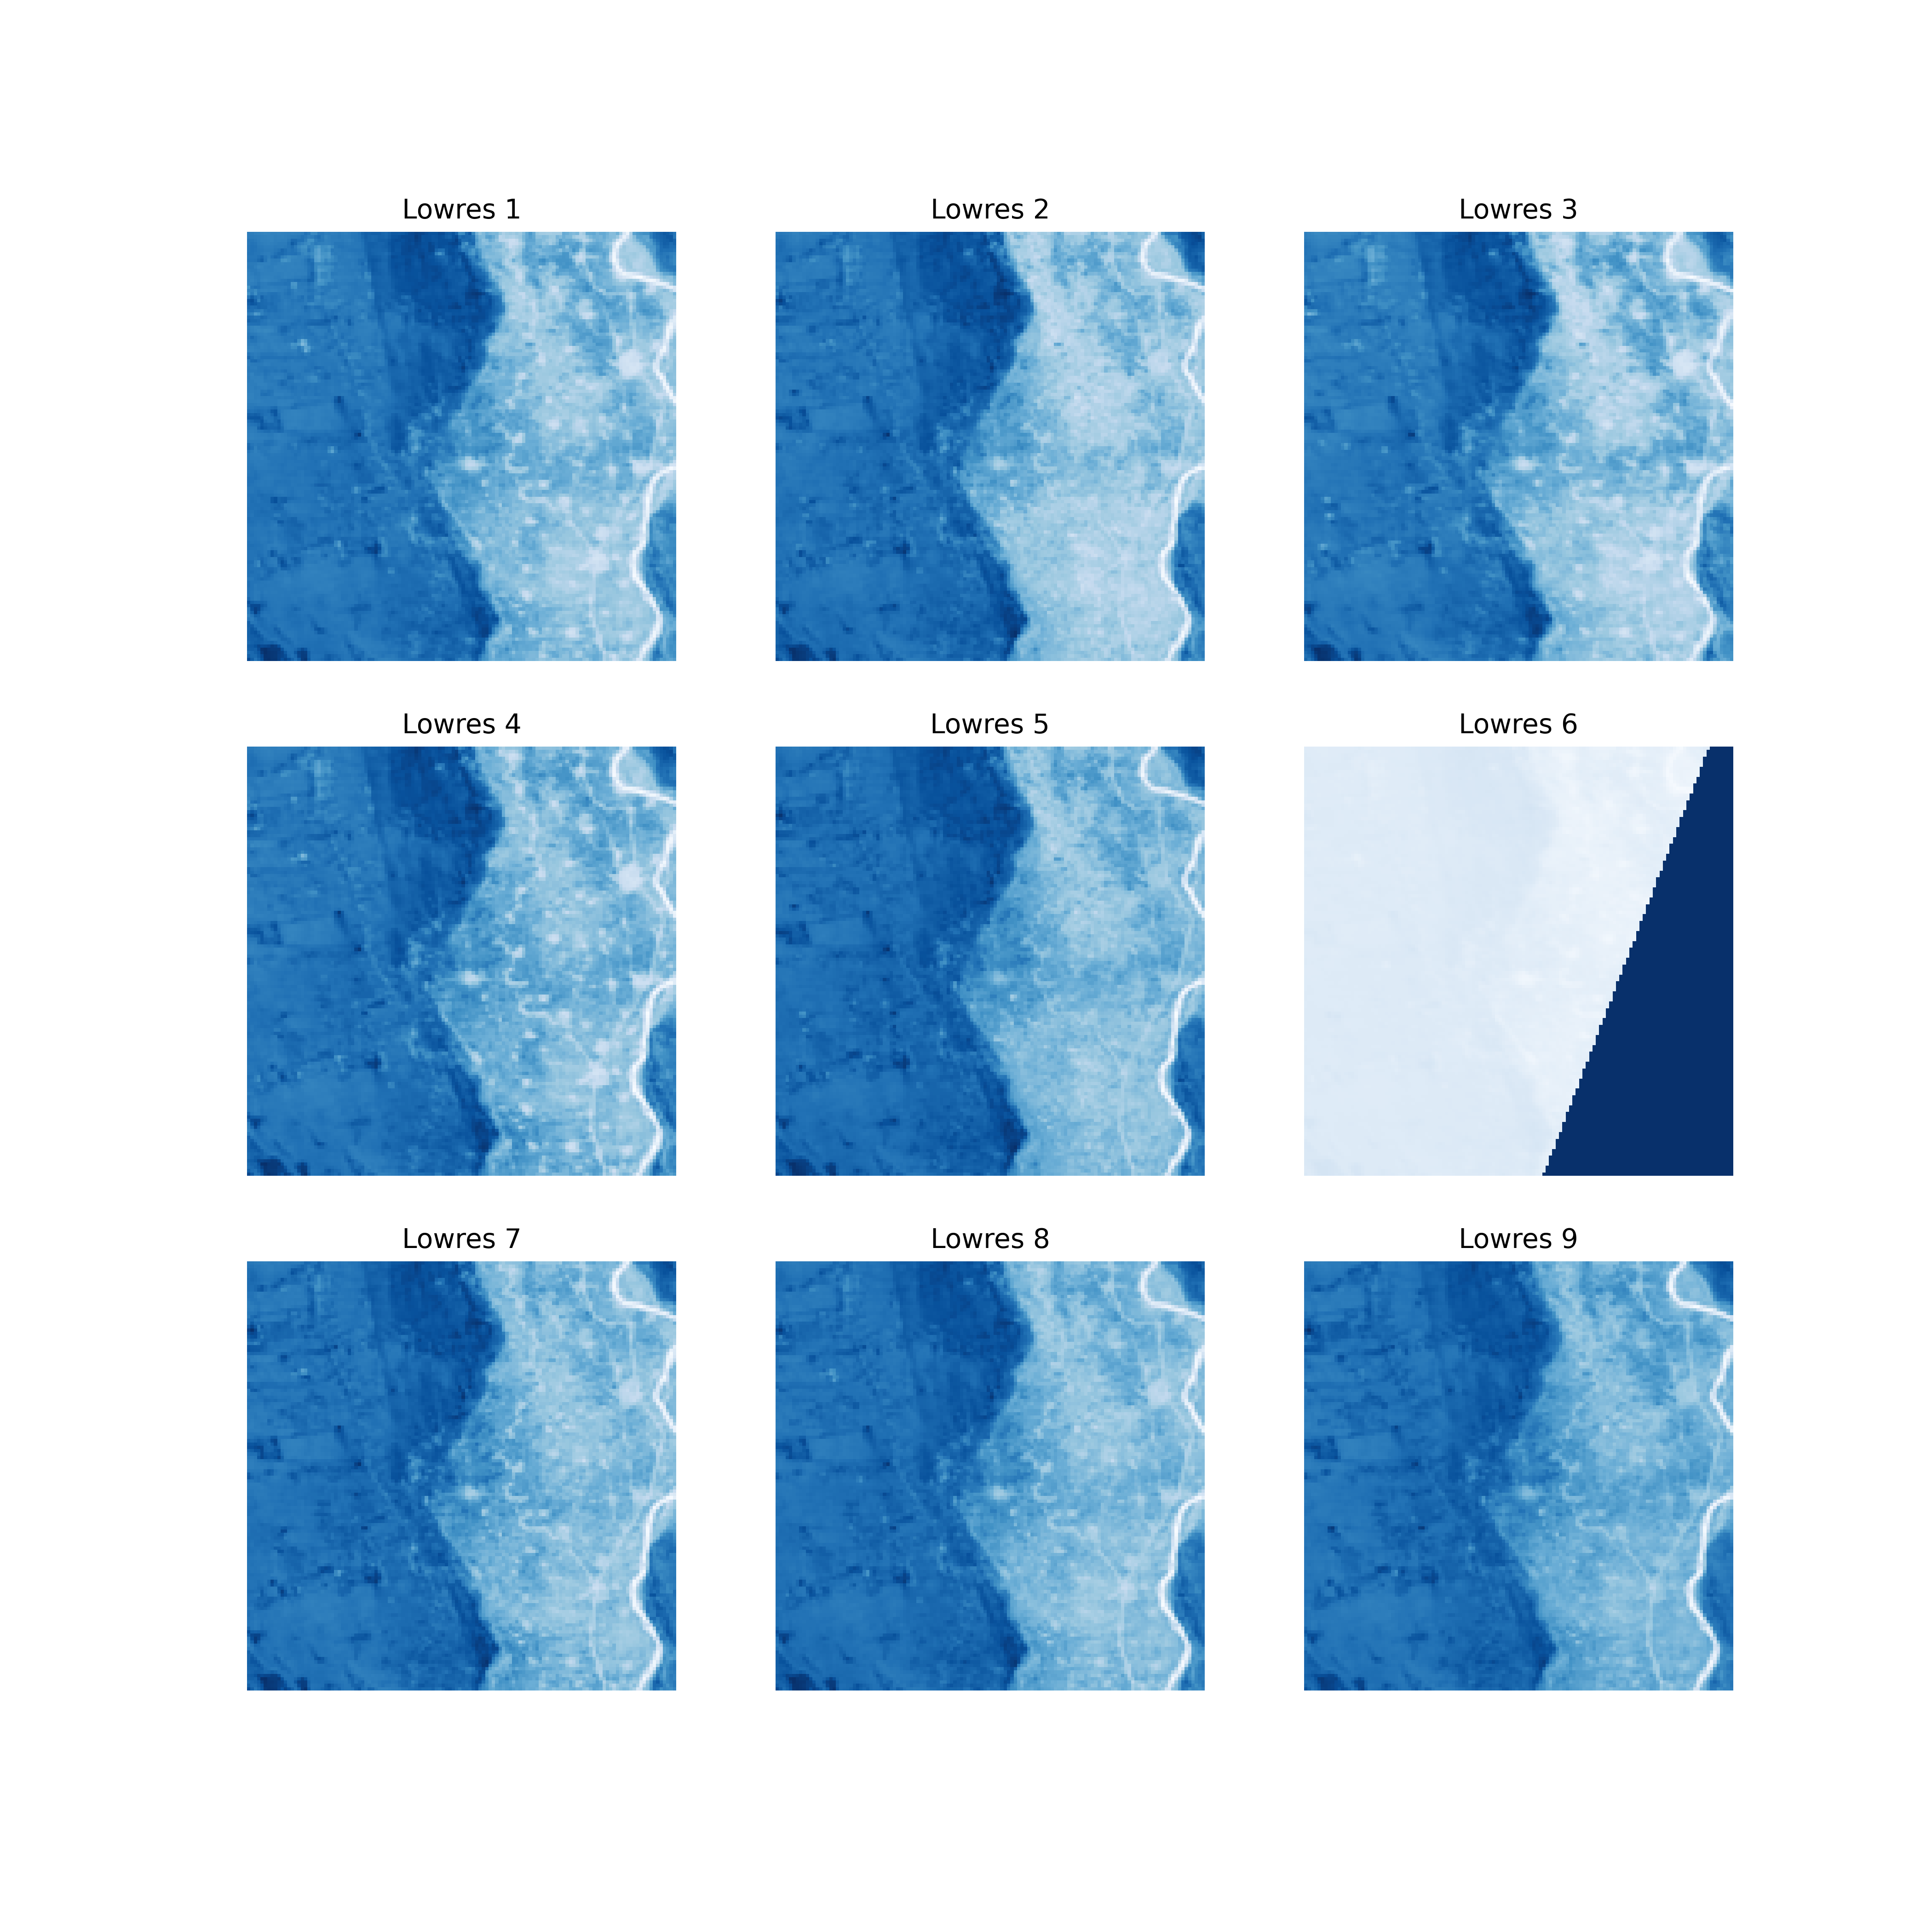
\includegraphics[width=0.4\textwidth]{low_res_inputs.png}
    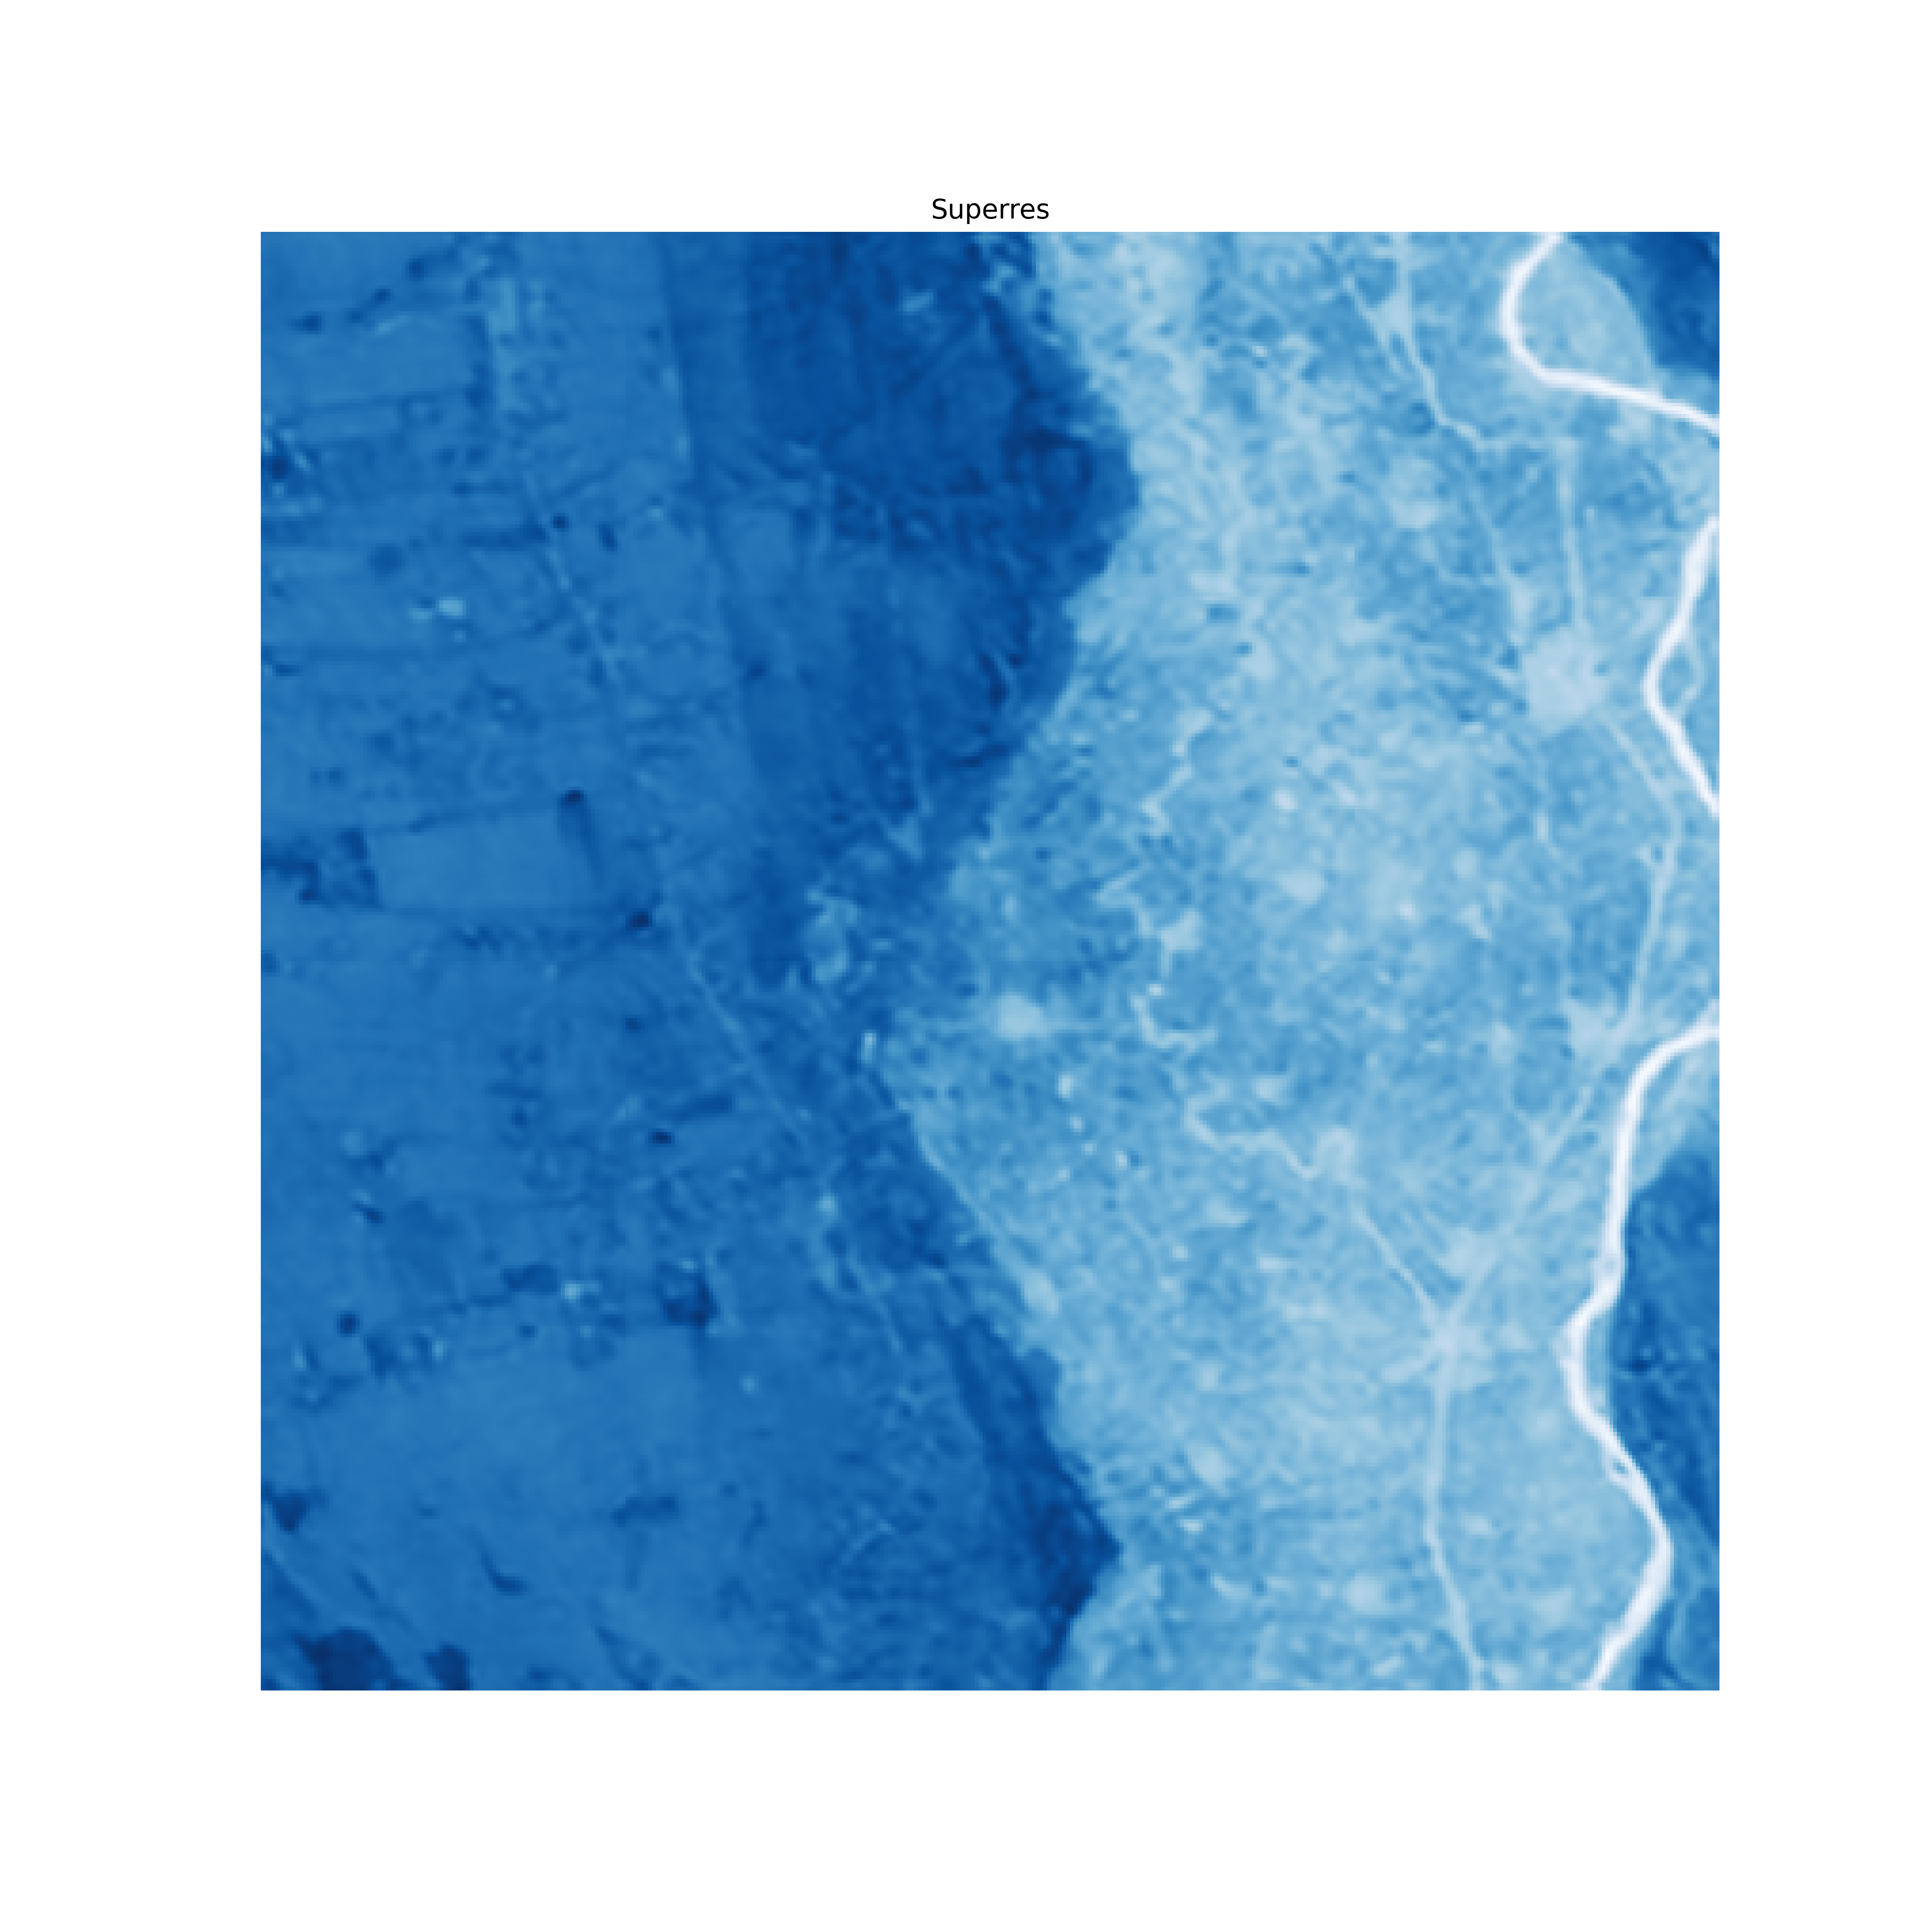
\includegraphics[width=0.4\textwidth]{super_res_output.png}
    \captionof{figure}{Low resolution (128x128) inputs from PROBA-V test data and generated 384x284 super resolved image.}
\end{center}


\section{Discussion}

As mentioned previously, one of the intended goals of this project was to integrate the WDSR3D network into a generative adversarial network for fine-tuning--a technique which has shown promising results for super resolution tasks. What is most salient about the technique is that it allows one to "add" an additional loss function to the model to further improve its results. In this case, the proposal was to add a notion of perceptual loss, which involves the comparison of features extracted from a pre-trained VGG network added to a weighted generator loss \citep{Ledig2016}. 

However, our implementation of the GAN and fine-tuning framework ran into a few snags. Primarily, we found that, when combined, the forward pass of the GAN was not automatically differentiable, if it was differentiable at all. Therefore, Tensorflow's automatic differentiation was unable to calculate the network gradient for either the generator or discriminator of the network. Attempts to debug the current implementation were unsuccessful, and any further attempts probably warrant a complete rewrite of this portion to split up the training of the generator and discriminator into separate function scopes. The likely culprit here is probably some combination of our generator, the WDSR-3D network implemented here, which has a complex input (an image set for the main path and a mean image for the residual path) and the complex loss function.

Another possible place for experimentation is to revisit the data augmentation step of the preprocessing. \citet{Dorr2020} and \citet{mark_bajo_2020_3733116} both attributed the performance of their model not to the architecture but to the data augmentation steps that preceded it. A possible modification that could be experimented with would be to undo the shuffling of the patches and instead to treat the frames as sequential allowing for a spatial \textit{and} temporal fusion of the low resolution images more in line with how video super resolution is accomplished. 

\section{Conclusion}

While not attaining the goals set out in the proposal, the project successfully implemented and replicated the results of using a WDSR-3D network on the PROBA-V dataset to produce superresolved 384x384 pixel images from a set of low-resolution 128x128 images. The attempt to set up a more complicated generative adversarial network also necessitated a much closer familiarity with Tensorflow documentation and how it achieves automatic differentiation. 

\bibliographystyle{unsrtnat}
\bibliography{references}

\end{document}